\documentclass[10pt, a4j, dvipdfmx]{jarticle}
\usepackage{titlesec}
\usepackage[dvipdfmx]{graphicx}
\usepackage[dvipdfmx]{color}
\usepackage{float}
\usepackage{wrapfig}
\usepackage{subfigure}
\usepackage{caption}

\graphicspath{{../images/}}

\makeatletter
\newcommand{\figcaption}[1]{\def\@captype{figure}\caption{#1}}
\newcommand{\tblcaption}[1]{\def\@captype{table}\caption{#1}}
\makeatother

\title{トランジスタ増幅}
\author{4年 電子システム工学科 40番  山地 駿徹}


\begin{document}

    \begin{center}
        \LARGE トランジスタの静特性
    \end{center}

    \section*{入力特性の測定方法}
    エミッタ接地回路で,$V_{CE}$を一定に保ち,$V_{BE}$を変化させたときの$I_B$の変化を測定する.
    \begin{figure}[H]
        \begin{minipage}{0.5\hsize}
            \centering
            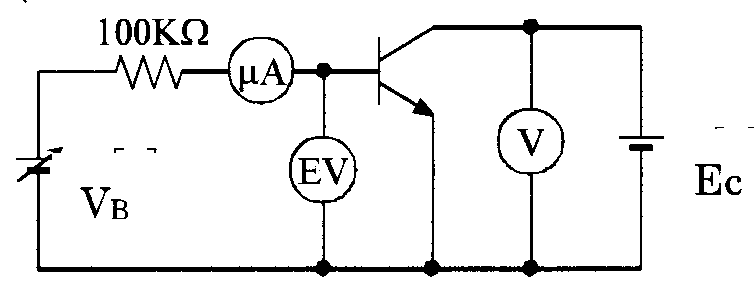
\includegraphics[width=50mm]{fig-1.png}
            \caption{入力特性測定回路}
            \label{fig:1}
        \end{minipage}
        \begin{minipage}{0.5\hsize}
            \centering
            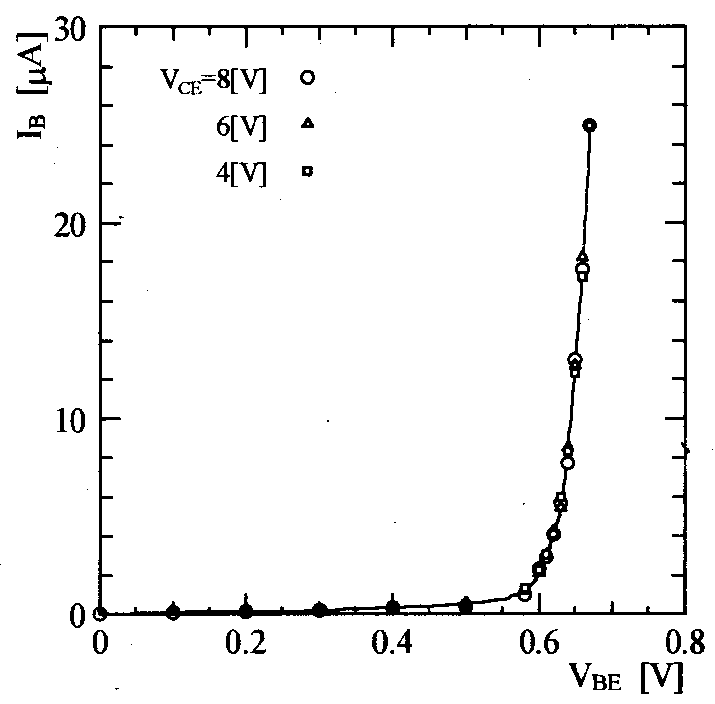
\includegraphics[height=45mm]{fig-2.png}
            \caption{入力特性}
            \label{fig:2}
        \end{minipage}
    \end{figure}

    \section*{出力特性の測定方法}
    エミッタ接地回路で,$I_B$を一定に保ち,$V_{CE}$を変化させたときの$I_C$の変化を測定する.
    \begin{figure}[H]
        \begin{minipage}{0.5\hsize}
            \centering
            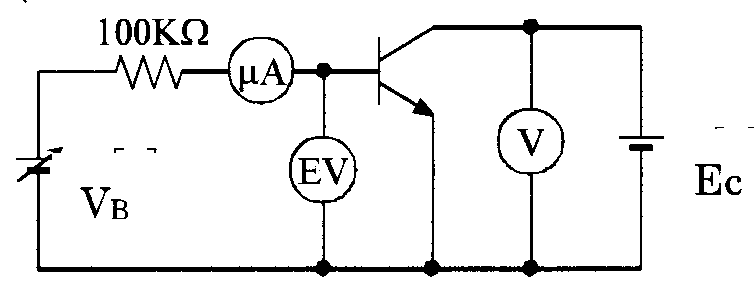
\includegraphics[width=50mm]{fig-1.png}
            \caption{出力特性測定回路}
            \label{fig:3}
        \end{minipage}
        \begin{minipage}{0.5\hsize}
            \centering
            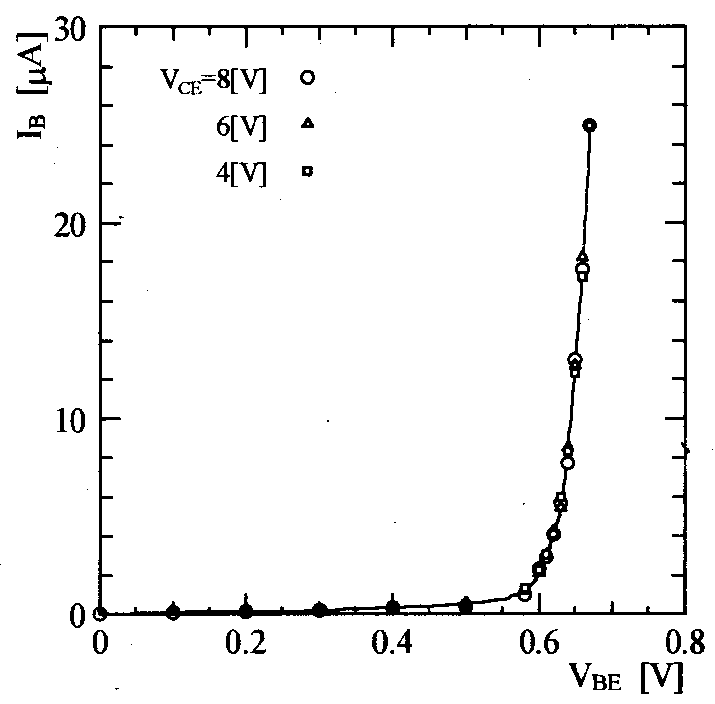
\includegraphics[height=45mm]{fig-2.png}
            \caption{出力特性}
            \label{fig:4}
        \end{minipage}
    \end{figure}
    \section*{吟味事項}
    \begin{enumerate}
        \item 電圧計,電流計の等級と内部抵抗を調べる.\\電圧計,電流計の接続方法により,計器の内部抵抗による測定誤差について考察する.\\その時の補正方法を考察する.
        \item $V_{CE} = 4[V]$,$I_B = 20[\mu A]$のときの$h$定数を,測定した特性図より求める.
    \end{enumerate}

    \newpage
    \begin{center}
        \LARGE トランジスタ増幅
    \end{center}

    \section*{電流増幅特性の測定方法}
    エミッタ接地回路で$R_C = 1[k\Omega]$を接続し$E_C = 8[V]$一定として,$I_B$を変化させたときの$I_C$の変化を測定する.
    \small (注. 電流計の内部抵抗が負荷抵抗に加算されないように$E_C$を調整する)
    \begin{figure}[H]
        \begin{minipage}{0.5\hsize}
            \centering
            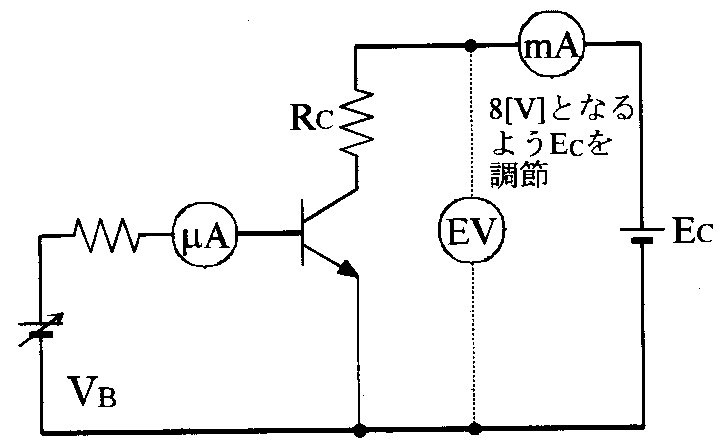
\includegraphics[width=50mm]{fig-5.png}
            \caption{電流増幅特性測定回路}
            \label{fig:5}
        \end{minipage}
        \begin{minipage}{0.5\hsize}
            \centering
            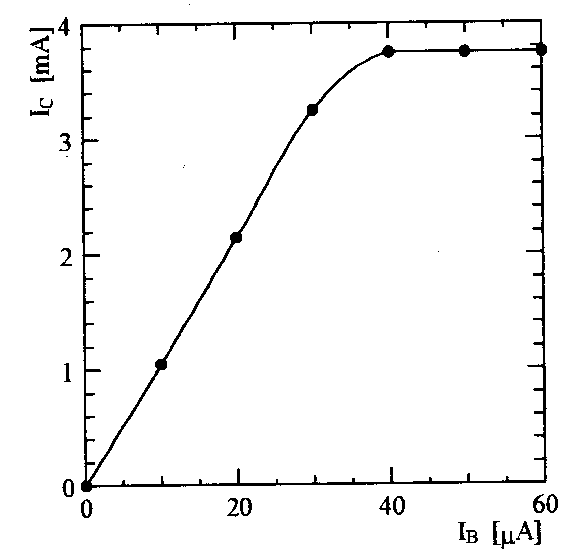
\includegraphics[height=45mm]{fig-6.png}
            \caption{電流増幅特性}
            \label{fig:6}
        \end{minipage}
    \end{figure}

    \section*{電圧増幅特性の測定方法}
    エミッタ接地回路で$R_C = 1[k\Omega]$を接続し$E_C = 8[V]$一定として,$V_{BE}$を変化させたときの$V_{CE}$の変化を測定する.
    \begin{figure}[H]
        \begin{minipage}{0.5\hsize}
            \centering
            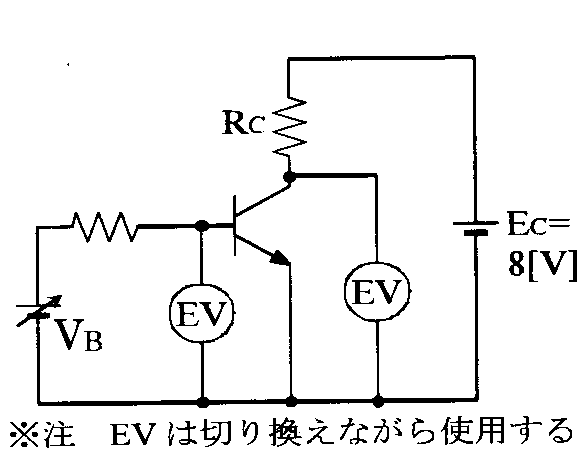
\includegraphics[width=50mm]{fig-7.png}
            \caption{電圧増幅特性測定回路}
            \label{fig:7}
        \end{minipage}
        \begin{minipage}{0.5\hsize}
            \centering
            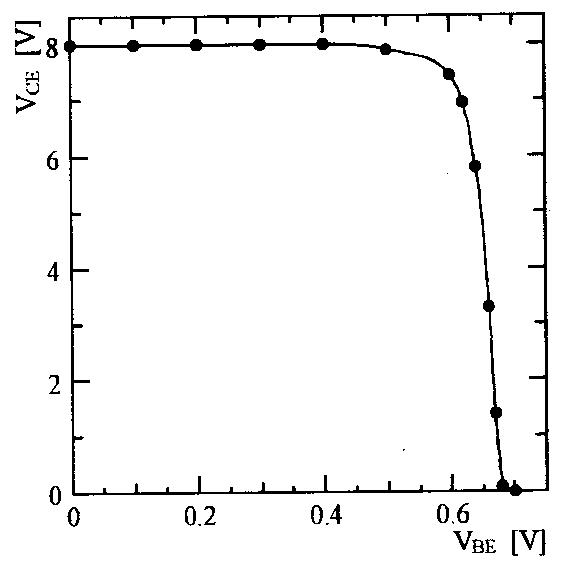
\includegraphics[height=45mm]{fig-8.png}
            \caption{電圧増幅特性}
            \label{fig:8}
        \end{minipage}
    \end{figure}

    以上の測定はトランジスタ増幅回路の交流不可線上の特性を測定することと等価である.\\
    まず,動作点$Q$を電流増幅特性の直線部分より決定する.次に,この動作点に対応する電圧増幅特性での動作点を記入する.

    \section*{吟味事項}
    \begin{enumerate}
        \item 電流増幅特性より,$h_{FE}$を求める.
        \item 電圧増幅特性より電圧増幅度を求める.
    \end{enumerate}

    \newpage
    \section*{直流バイアス回路定数の選定及びバイアス電圧測定}

\end{document}